%=================================================================
% fp-tools BioMedInformatics manuscript
% Compile with: latexmk -pdf main.tex   (or pdflatex x3)
% Requires the MDPI class shipped under Definitions/ (extracted from
% paper/MDPI_template_ACS.zip by paper/scripts/prepare_biomedinformatics_template.py)
%=================================================================
\documentclass[biomedinformatics,article,submit,pdftex,moreauthors]{Definitions/mdpi}

% MDPI internal commands - do not modify
\firstpage{1}
\makeatletter
\setcounter{page}{\@firstpage}
\makeatother
\pubvolume{1}
\issuenum{1}
\articlenumber{0}
\pubyear{2026}
\copyrightyear{2026}
\datereceived{ }
\dateaccepted{ }
\datepublished{ }

%------------------------------------------------------------------
\Title{fp-tools: A Reproducible Command-Line Platform for Classical
and Multiscale ATAC-seq Footprinting, Supervised TF-Binding Prediction,
Motif Discovery, and Variant Scoring}

\Author{Yaoxiang Li $^{1}$ and Chunling Yi $^{1,}$*}

\AuthorNames{Yaoxiang Li and Chunling Yi}

\address{%
$^{1}$ \quad Department of Oncology, Lombardi Comprehensive Cancer Center, Georgetown University Medical Center, Georgetown University, Washington, DC, USA; yl814@georgetown.edu (Y.L.); chunling.yi@georgetown.edu (C.Y.)}

\corres{Correspondence: chunling.yi@georgetown.edu (C.Y.)}

\abstract{(1) Background: Transcription-factor (TF) footprinting from ATAC-seq is
central to inferring regulatory activity, but the surrounding ecosystem is
fragmented across single-purpose tools with heterogeneous interfaces,
inconsistent reproducibility, and uneven test coverage, which raises the cost of
building end-to-end regulatory-genomics analyses. (2) Methods: We present
\texttt{fp-tools}, a standalone, pip-installable Python package that unifies bias
correction, footprint scoring, differential TF-binding detection, and aggregate
visualization behind stable command-line entry points, with optional YAML and
graphical wrappers. Around this core we add explicitly opt-in scientific modules:
multiscale and nucleosome-aware scoring, motif-centric supervised TF-binding
prediction, motif-relaxed and motif-free candidate recovery, de novo motif
discovery orchestration, footprint-aware variant scoring, single-cell pseudobulk
aggregation, replicate-aware differential-binding uncertainty reporting, and a
competition-aware decomposition of overlapping TF-scale and nucleosome-scale
footprint signals. (3) Results: The package provides deterministic,
regression-tested workflows; a tiered public-data benchmark design with AUROC,
AUPRC, recall-at-FDR, calibration, and bootstrap-confidence-interval metrics; and
paper-ready figure generators. In a chromosome-4 ENCODE pilot benchmark spanning
three cell lines and 12 cell--TF tasks, an integrated \texttt{fp-tools} score
combining accessibility, motif strength, GC content, and available cut-site
footprint features achieved the highest AUROC among the evaluated predictors in
every task (mean AUROC $0.80$), compared with motif-only scoring ($0.77$), raw
accessibility ($0.52$), and footprint-only scoring where available ($0.55$). The
same pilot shows that footprint occupancy is recoverable only at Tn5 cut-site
resolution (AUROC $0.68$) and not from smoothed coverage ($0.24$). New modules
preserve the behavior of the classical commands when they are not invoked. (4)
Conclusions: \texttt{fp-tools} integrates
established footprinting strengths with modern multiscale, supervised, and
variant-oriented extensions in a single reproducible package, lowering the barrier
to standardized, benchmarkable ATAC-seq regulatory analysis.}

\keyword{ATAC-seq; transcription factor footprinting; chromatin accessibility;
motif analysis; supervised TF-binding prediction; multiscale footprints;
variant scoring; reproducibility; command-line bioinformatics}

\begin{document}

%==================================================================
\section{Introduction}
%==================================================================

Chromatin accessibility profiling by the assay for transposase-accessible
chromatin using sequencing (ATAC-seq) has become a standard readout of the active
regulatory landscape of a cell~\cite{buenrostro2013}. Within accessible regions,
sequence-specific transcription factors (TFs) protect the DNA they occupy from
transposition, leaving characteristic depletions---``footprints''---flanked by
hyper-accessible edges. Detecting and interpreting these footprints supports
inference of TF occupancy, differential regulation between conditions, and the
functional consequences of non-coding variation.

A mature but \emph{fragmented} ecosystem of methods addresses pieces of this
problem. Classical footprinting and differential-binding frameworks such as
TOBIAS~\cite{bentsen2020} and HINT-ATAC~\cite{li2019hint} correct enzymatic
sequence bias and score footprints at a single TF-relevant scale. Multiscale and
nucleosome-aware approaches, exemplified by the PRINT/scPrinter
family~\cite{hu2024print}, model accessibility structure across a range of
footprint widths. Supervised TF-binding-site (TFBS) predictors such as
maxATAC~\cite{cazares2023maxatac} and sequence-to-profile models such as
ChromBPNet~\cite{chrombpnet2024} learn occupancy from labeled data or raw
sequence, and downstream interpretation tools and variant scorers translate models
into motif and allele-level effects. Each tool typically ships its own interface,
input conventions, and assumptions, so assembling a coherent, reproducible
pipeline---and \emph{benchmarking} alternatives on common ground---remains
laborious and error-prone.

Three practical gaps motivate this work. First, \textbf{interface fragmentation}:
moving from bias correction to footprint scoring to differential binding to
visualization commonly spans several packages with incompatible I/O. Second,
\textbf{reproducibility and testing}: many footprinting workflows lack
deterministic regression tests, pinned environments, and machine-checkable output
contracts, making it hard to know whether a change altered results. Third,
\textbf{extensibility without regression}: adding new scientific behavior (e.g.,
multiscale scoring or supervised prediction) often forces users onto entirely new
tools rather than extending a stable base.

We address these gaps with \texttt{fp-tools}, a standalone Python package that
(i) provides stable, primary command-line entry points for the four core
workflows---bias correction, footprint scoring, differential TF-binding
detection, and aggregate plotting; (ii) layers optional YAML- and GUI-based
wrappers without displacing the command line; and (iii) introduces a series of
\emph{explicitly opt-in} scientific modules that extend the platform while leaving
the classical commands unchanged when they are not invoked. The guiding principle
is conservative: keep existing bulk ATAC workflows stable and reproducible, and
add novelty as composable modules with their own tests, documentation, and
benchmark hooks. This paper describes the package architecture, the new modules,
the tiered benchmarking and figure-generation design, and the reproducibility
engineering that ties them together.

%==================================================================
\section{Materials and Methods}
%==================================================================

\subsection{Package Architecture and Core Workflows}

\texttt{fp-tools} is distributed as a pip-installable package (\texttt{fp-tools-bio})
with vendored Cython internals for performance-critical signal operations. Core
scientific tools live under a single namespace and are exposed through stable
console entry points. The four primary commands are:
\begin{itemize}
  \item \texttt{atac-correct} --- Tn5 sequence-bias correction producing corrected
        and expected/bias bigWig tracks and a QC report;
  \item \texttt{score-footprints} --- footprint, sum, mean, and pass-through
        scoring modes over corrected signal within regions;
  \item \texttt{detect-tf-binding} --- motif-anchored differential binding across
        one or more conditions, with repeated-condition replicate grouping and a
        skewness report for multi-condition runs;
  \item \texttt{plot-aggregate} --- aggregate footprint visualization from single
        BED files or directories, with control overlays, fixed-grid layouts,
        labels, and CSV exports.
\end{itemize}
Legacy aliases (\texttt{ATACorrect}, \texttt{FootprintScores}, \texttt{ScoreBigwig},
\texttt{BINDetect}, \texttt{PlotAggregate}) are retained for backward
compatibility. A YAML runner (\texttt{fp-tools-run}) expands declarative configs
into the same commands, and an optional Streamlit GUI (\texttt{fp-tools-gui})
provides forms, run history, and output discovery. Direct CLI usage is the primary
interface; YAML and GUI are wrappers that never replace it.

For classical footprint scoring, let $x_i$ denote corrected Tn5 cut-site signal
around candidate position $p$. The default footprint score is a center-versus-flank
contrast,
\[
F(p)=\frac{1}{|L|+|R|}\left(\sum_{i\in L}x_i+\sum_{i\in R}x_i\right)-
\frac{1}{|C|}\sum_{i\in C}x_i,
\]
where $C$ is the protected center and $L$ and $R$ are flanking windows. Larger
values therefore correspond to the expected footprint pattern: fewer cuts at the
putative bound site and more cuts in nearby accessible flanks.

\subsection{Opt-in Scientific Modules}

New behavior is added as separate modules, each with its own console script,
unit tests, and documentation, and each inert unless explicitly invoked:
\begin{itemize}
  \item \emph{Multiscale and nucleosome-aware scoring}: \texttt{score-footprints
        --score multiscale} computes depletion across a configurable set of scales
        (default 8--147~bp), with \texttt{max}/\texttt{mean} scale collapse, an
        optional summary bigWig, and a compressed NPZ tensor sidecar
        (\texttt{--output-multiscale-npz}) of shape $n_\text{scales}\times
        \text{positions}$ for downstream visualization.
  \item \emph{Supervised TFBS prediction}: \texttt{fp-tools-build-tfbs-features}
        assembles motif-centric feature tables (genome GC, multiscale/signal
        summaries, optional overlap labels); \texttt{fp-tools-train-tfbs-model}
        and \texttt{fp-tools-predict-tfbs} train and apply tabular models with
        saved bundles and calibration metrics.
  \item \emph{Motif-relaxed and motif-free recovery}:
        \texttt{fp-tools-generate-candidates} nominates candidates from score
        bigWigs and peaks without requiring motif hits, with an optional
        lower-threshold motif-BED merge path; \texttt{fp-tools-rerank-candidates}
        integrates candidate, motif, family, and model scores into a ranked site
        table with provenance.
  \item \emph{De novo motif discovery}: \texttt{fp-tools-export-candidate-fasta},
        \texttt{fp-tools-meme-command}, and \texttt{fp-tools-motif-discovery-plan}
        export candidate-centered FASTA and emit reproducible MEME/DREME, Tomtom,
        and summary command plans; \texttt{fp-tools-summarize-motifs} parses
        MEME/Tomtom output into TSV and HTML reports with inline consensus logos.
  \item \emph{Footprint-aware variant scoring}: \texttt{fp-tools-score-variants}
        performs genome reference checks, candidate-overlap annotation,
        deterministic ref/alt sequence-context deltas, optional JASPAR/MEME PWM
        ref/alt motif deltas, and optional tabular-model probability deltas.
  \item \emph{Pseudobulk aggregation}: \texttt{fp-tools-pseudobulk} groups
        single-cell ATAC fragments by annotation columns into pseudobulk fragment
        files, TSV/YAML manifests, and downstream command plans.
  \item \emph{Replicate-aware differential-binding reporting}:
        \texttt{fp-tools-bindetect-replicate-report} (this work) summarizes a
        BINDetect \texttt{*\_results.txt} table into per-comparison effect sizes,
        $p$-values, replicate support category, and a $p$-value--derived
        uncertainty model (Section~\ref{sec:replicate}).
  \item \emph{Competition-aware footprint decomposition}:
        \texttt{fp-tools-decompose-competition} (this work) decomposes multiscale
        signal into competing TF-scale and nucleosome-scale components
        (Section~\ref{sec:competition}).
\end{itemize}

\subsection{Replicate-aware Differential-Binding Uncertainty}
\label{sec:replicate}

BINDetect-style result tables report, per motif and comparison, an aggregate
effect size (\texttt{change}) and a two-sided $p$-value, but not per-replicate
scores. We infer replicate counts $n_c$ per condition from (in order of priority)
an explicit \texttt{condition}/\texttt{n\_replicates} or
\texttt{condition}/\texttt{replicate} map, \texttt{<condition>\_n\_replicates}
columns in the result table, or a single-replicate fallback. Each comparison is
labeled \texttt{replicate-supported} when $\min(n_1,n_2)\ge 2$ and
\texttt{single-replicate} otherwise. To attach uncertainty we recover an
approximate standard error from the reported $p$-value, $\mathrm{SE} =
|\text{change}|/z$ with $z = \Phi^{-1}(1-p/2)$, and report a replicate-shrunk
effect $\widehat{\text{change}} = w\cdot\text{change}$ with shrinkage weight
$w = n_\text{min}/(n_\text{min}+1)$ that grows toward~1 with replicate support,
together with a 95\% interval $\text{change}\pm 1.96\,\mathrm{SE}$. The tool emits
a per-comparison long-form table, a comparison-level summary (significant-motif
counts, median effect SE, mean shrinkage weight), and an optional diagnostic
figure.

\subsection{Competition-aware Overlap Decomposition}
\label{sec:competition}

Overlapping regulatory elements produce footprint signals at multiple scales
simultaneously: short TF-scale depletions can coincide with wider
nucleosome-scale structure. Using the multiscale NPZ tensor, we partition scales
into a TF-scale band (default 3--30~bp) and a nucleosome-scale band (default
120--200~bp), and collapse each band to a positionwise non-negative profile
$t$ and $n$ by taking the per-position maximum over band scales. We then
decompose the signal additively at each position into shared (competing),
TF-only, and nucleosome-only components,
\[
\text{shared} = \min(t,n),\quad
\text{tf\_only} = t-\text{shared},\quad
\text{nuc\_only} = n-\text{shared},
\]
and integrate over the region. A \emph{competition index} is the shared fraction
of total signal, $\text{shared}_\text{AUC}/(\text{tf\_only}_\text{AUC}+
\text{nuc\_only}_\text{AUC}+\text{shared}_\text{AUC})$, and each region is labeled
by its dominant component (\texttt{tf}, \texttt{nucleosome}, \texttt{competing},
or \texttt{none}). The tool emits per-region and dataset-level tables and an
optional figure.

\subsection{Public Data, Benchmark Tiers, and Metrics}

Benchmarks are organized as versioned TSV manifests recording source, benchmark
tier, cell type, donor, TF, assay, accessions, assembly, output type, format,
URL, checksum, status, local path, split, and notes. A discovery script queries
the ENCODE REST API for released human GRCh38 ATAC-seq and matched TF
ChIP-seq/CUT\&RUN; a resumable downloader writes per-benchmark download reports
with checksums and local paths. Raw and processed public data, and large
benchmark outputs, are kept out of version control; scripts, manifests, schemas,
tiny fixtures, and figure code are tracked.

The benchmark is deliberately \emph{tiered} rather than monolithic
(Table~\ref{tab:tiers}): a fast CI-smoke tier on tiny fixtures; a bulk matched
tier (ENCODE bulk ATAC vs. matched TF ChIP/CUT\&RUN) as the primary classical
benchmark; a depth-robustness tier over downsampled ATAC; a motif-removal tier for
motif-relaxed/free and de novo validation; a supervised-TFBS tier; a variant tier;
and a later pseudobulk tier. For binary TF-binding labels we compute AUROC and
AUPRC globally and per TF-cell task, recall at 1\%, 5\%, and 10\% FDR, precision at
fixed recall, calibration curves with expected and maximum calibration error,
Brier score for probability models, per-TF macro averages, Wilcoxon signed-rank
tests for paired method comparisons, and stratified bootstrap confidence intervals
for key deltas. Metric, calibration, and bootstrap computations are implemented as
standalone, unit-tested scripts and combined by a benchmark pipeline runner that
also emits PDF/SVG/PNG figure panels.

\begin{table}[H]
\caption{Tiered benchmark design. Large data and outputs are untracked; only
manifests, scripts, and small smoke results are committed.\label{tab:tiers}}
\newcolumntype{Y}{>{\raggedright\arraybackslash}X}
\begin{tabularx}{\textwidth}{lYY}
\toprule
\textbf{Tier} & \textbf{Purpose} & \textbf{Primary outputs}\\
\midrule
CI smoke & Install/regression checks on tiny fixtures & command success, output existence, stable summaries\\
Bulk matched & Main classical benchmark (ATAC vs. matched TF ChIP/CUT\&RUN) & TFBS labels, predictions, AUROC/AUPRC, reports\\
Depth robustness & Shallow-depth sensitivity (50/25/10/5\%) & performance-vs-depth and calibration curves\\
Motif removal & Motif-relaxed/free and de novo validation & recovered ChIP-supported sites, rediscovered-motif stats\\
Supervised TFBS & Tabular model benchmark & probability metrics, calibration, comparator tables\\
Variant & Translational benchmark (caQTL/allele-specific) & delta-score enrichment, case studies\\
Pseudobulk & Single-cell extension & cell-type TF programs, group comparisons\\
\bottomrule
\end{tabularx}
\end{table}

\subsection{Reproducibility Engineering}

The package ships a unit-test suite covering numerical helpers, CLI behavior, and
deterministic golden CLI regressions for footprint scoring, differential binding,
and aggregate plotting, with an opt-in slow regression for bias correction. A
continuous-integration workflow runs the suite on a clean checkout using only
small fixtures. Every benchmark result is expected to store random seeds, tool
versions, command lines, and the resolved manifest. Figures are saved as vector
PDF/SVG plus 300-dpi PNG previews, with source plotting tables retained for
auditability.

%==================================================================
\section{Results}
%==================================================================

\subsection{A Unified, Reproducible Footprinting Platform}

\texttt{fp-tools} consolidates the four core ATAC footprinting workflows behind a
single, consistent command-line interface with shared region/signal conventions,
so a complete analysis---bias correction, footprint scoring, differential binding,
and aggregate visualization---runs without crossing package boundaries or
reformatting intermediates. The optional YAML runner reproduces any pipeline from
a declarative config, and the GUI exposes the same operations with run history and
output discovery for less command-line-oriented users. Because every wrapper
expands to the same underlying commands, results are identical across entry
points, and the YAML config doubles as a machine-readable record of the analysis.

\subsection{Deterministic Regression and CLI Coverage}

The classical commands are covered by deterministic golden regressions that pin
output summaries for footprint scoring, differential binding, and aggregate
plotting, plus CLI smoke tests for all public and legacy entry points and YAML
dry-runs. This converts ``did this change alter results?'' from a manual judgment
into an automatically checked contract, and provides the stable base on which the
opt-in modules are layered without disturbing default behavior.

\subsection{Multiscale and Nucleosome-aware Extension}

The multiscale module augments single-scale footprint scoring with a
scale-by-position view of accessibility depletion. The compressed NPZ tensor
sidecar serves both as a paper-figure input and as the substrate for the
competition decomposition. On synthetic constructs, narrow TF-scale and broad
nucleosome-scale depletions are recovered at their respective scales, and the
companion aggregate visualization (scale-by-position heatmap, collapsed profile,
and per-scale means) renders these directly. Crucially, default single-scale
scoring is unchanged unless multiscale mode is requested.

\subsection{Supervised, Motif-relaxed, De novo, and Variant Modules}

The supervised TFBS path turns candidate sites into motif-centric feature tables
and trains reproducible tabular models with saved bundles and calibration
outputs, providing a labeled-data complement to classical scoring. The
motif-relaxed/free path recovers candidate sites from signal alone or from
lower-threshold motif merges and reranks them with motif-family and model
evidence, enabling recovery of occupancy that strict motif thresholds miss. The de
novo path orchestrates reproducible MEME/DREME and Tomtom command plans and
summarizes results into TSV/HTML reports with inline consensus logos. The variant
module annotates alleles with reference checks, candidate overlap, deterministic
sequence-context deltas, optional PWM ref/alt motif deltas, and optional model
probability deltas. Each module is independently tested and documented, and none
alters the classical commands when unused.

\subsection{Replicate-aware Uncertainty and Competition Decomposition}

The replicate-aware report adds an interpretable uncertainty layer to differential
binding: comparisons are categorized by replicate support, and effect sizes are
reported with a $p$-value--derived standard error, a replicate-driven shrinkage
weight, and confidence intervals, so single-replicate comparisons are flagged and
conservatively shrunk relative to replicate-supported ones. The competition
decomposition attributes overlapping footprint signal to TF-scale,
nucleosome-scale, and shared (competing) components per region, with a competition
index and a dominant-component label, surfacing loci where TF and nucleosome
occupancy compete rather than treating accessibility as single-scale.

\subsection{Benchmark and Figure Infrastructure}

The tiered benchmark design (Table~\ref{tab:tiers}), the
metric/calibration/bootstrap scripts, the label-overlap and motif-removal table
builders, and the pipeline runner together provide an executable path from public
ENCODE data to publication-ready metrics and figures. To demonstrate this path
end-to-end on real data, we benchmarked four scoring paradigms on ENCODE ATAC-seq
peaks restricted to chromosome~4, labeling each accessible region positive when it
overlaps a matched ChIP-seq peak for the target factor. The compared predictors
were raw accessibility magnitude, best JASPAR PWM motif log-odds score, cut-site
footprint occupancy at the best motif hit where ATAC BAM data were available, and
an integrated \texttt{fp-tools} score from out-of-fold logistic regression over
accessibility, motif score, local GC content, and available footprint features:
\[
\Pr(y=1\mid z)=\sigma(\beta_0+\beta_1 a+\beta_2 m+\beta_3 g+\beta_4 f),
\]
where $y$ denotes ChIP-supported binding, $a$ is accessibility, $m$ is motif score,
$g$ is GC content, and $f$ is the cut-site footprint score when available. Model
coefficients were learned within cross-validation, and performance was reported on
held-out folds. For tasks without BAM-derived cut-site footprints, the integrated
model used the available accessibility, motif, and GC features. We evaluated 12 cell--TF tasks:
six transcription factors in K562 (CTCF, GATA1, SPI1, REST, MAX, JUND;
$n=1{,}900$ accessible regions each), two in GM12878 (CTCF, SPI1; $n=9{,}482$),
and four in HepG2 (CTCF, MAX, JUND, REST; $n=8{,}068$).

In this chromosome-4 pilot, the integrated \texttt{fp-tools} score achieved the
highest AUROC among the evaluated predictors in all 12 tasks
(Table~\ref{tab:methods}, Figure~\ref{fig:method_multi}). Mean AUROC across tasks
was $0.52$ for accessibility, $0.77$ for motif-only scoring, and $0.80$ for the
integrated score. In K562 tasks with cut-site footprints, footprint-only signal
averaged $0.55$ AUROC: it was informative for CTCF but was not sufficient as a
standalone predictor across factors. Motif-only scoring remained a strong baseline,
especially for information-rich motifs such as CTCF and SPI1, but the integrated
model consistently matched or improved it. The largest gains over motif-only
scoring occurred for MAX and JUND, including K562 MAX ($0.74\rightarrow0.83$),
HepG2 MAX ($0.64\rightarrow0.75$), K562 JUND ($0.83\rightarrow0.87$), and HepG2
JUND ($0.63\rightarrow0.67$). These results support the intended role of
\texttt{fp-tools}: preserving interpretable classical predictors while providing a
reproducible route to combine sequence, accessibility, composition, and footprint
features when those data are available. Full AUROC/AUPRC values and bootstrap
confidence intervals are reported in the benchmark metrics table distributed with
the analysis outputs (see Data Availability). Whole-genome and chromosome-held-out
benchmarks are the next validation step before making broad superiority claims.

\begin{table}[H]
\caption{Integrated method-comparison pilot benchmark on ENCODE ATAC-seq peaks
(chromosome~4) labeled by matched ChIP-seq overlap. Values are AUROC point
estimates; the full metrics TSV contains AUPRC and 200-resample bootstrap 95\% CIs.
The footprint-only column is shown only where BAM-derived cut-site footprints were
computed.\label{tab:methods}}
\newcolumntype{Z}{>{\centering\arraybackslash}X}
\begin{tabularx}{\textwidth}{llZZZZ}
\toprule
\textbf{Cell / TF} & \textbf{Pos. frac.} & \textbf{Access.} & \textbf{Motif} & \textbf{Footprint} & \textbf{Integrated}\\
\midrule
K562 / CTCF & 0.36 & 0.53 & 0.87 & 0.68 & \textbf{0.88}\\
K562 / GATA1 & 0.08 & 0.58 & 0.72 & 0.53 & \textbf{0.73}\\
K562 / SPI1 & 0.28 & 0.47 & 0.79 & 0.54 & \textbf{0.79}\\
K562 / REST & 0.06 & 0.48 & 0.72 & 0.56 & \textbf{0.73}\\
K562 / MAX & 0.49 & 0.44 & 0.74 & 0.56 & \textbf{0.83}\\
K562 / JUND & 0.08 & 0.59 & 0.83 & 0.41 & \textbf{0.87}\\
\midrule
GM12878 / CTCF & 0.26 & 0.57 & 0.90 & -- & \textbf{0.90}\\
GM12878 / SPI1 & 0.28 & 0.50 & 0.78 & -- & \textbf{0.78}\\
\midrule
HepG2 / CTCF & 0.28 & 0.59 & 0.86 & -- & \textbf{0.87}\\
HepG2 / MAX & 0.35 & 0.49 & 0.64 & -- & \textbf{0.75}\\
HepG2 / JUND & 0.13 & 0.49 & 0.63 & -- & \textbf{0.67}\\
HepG2 / REST & 0.006 & 0.51 & 0.81 & -- & \textbf{0.86}\\
\bottomrule
\end{tabularx}
\end{table}

\begin{figure}[H]
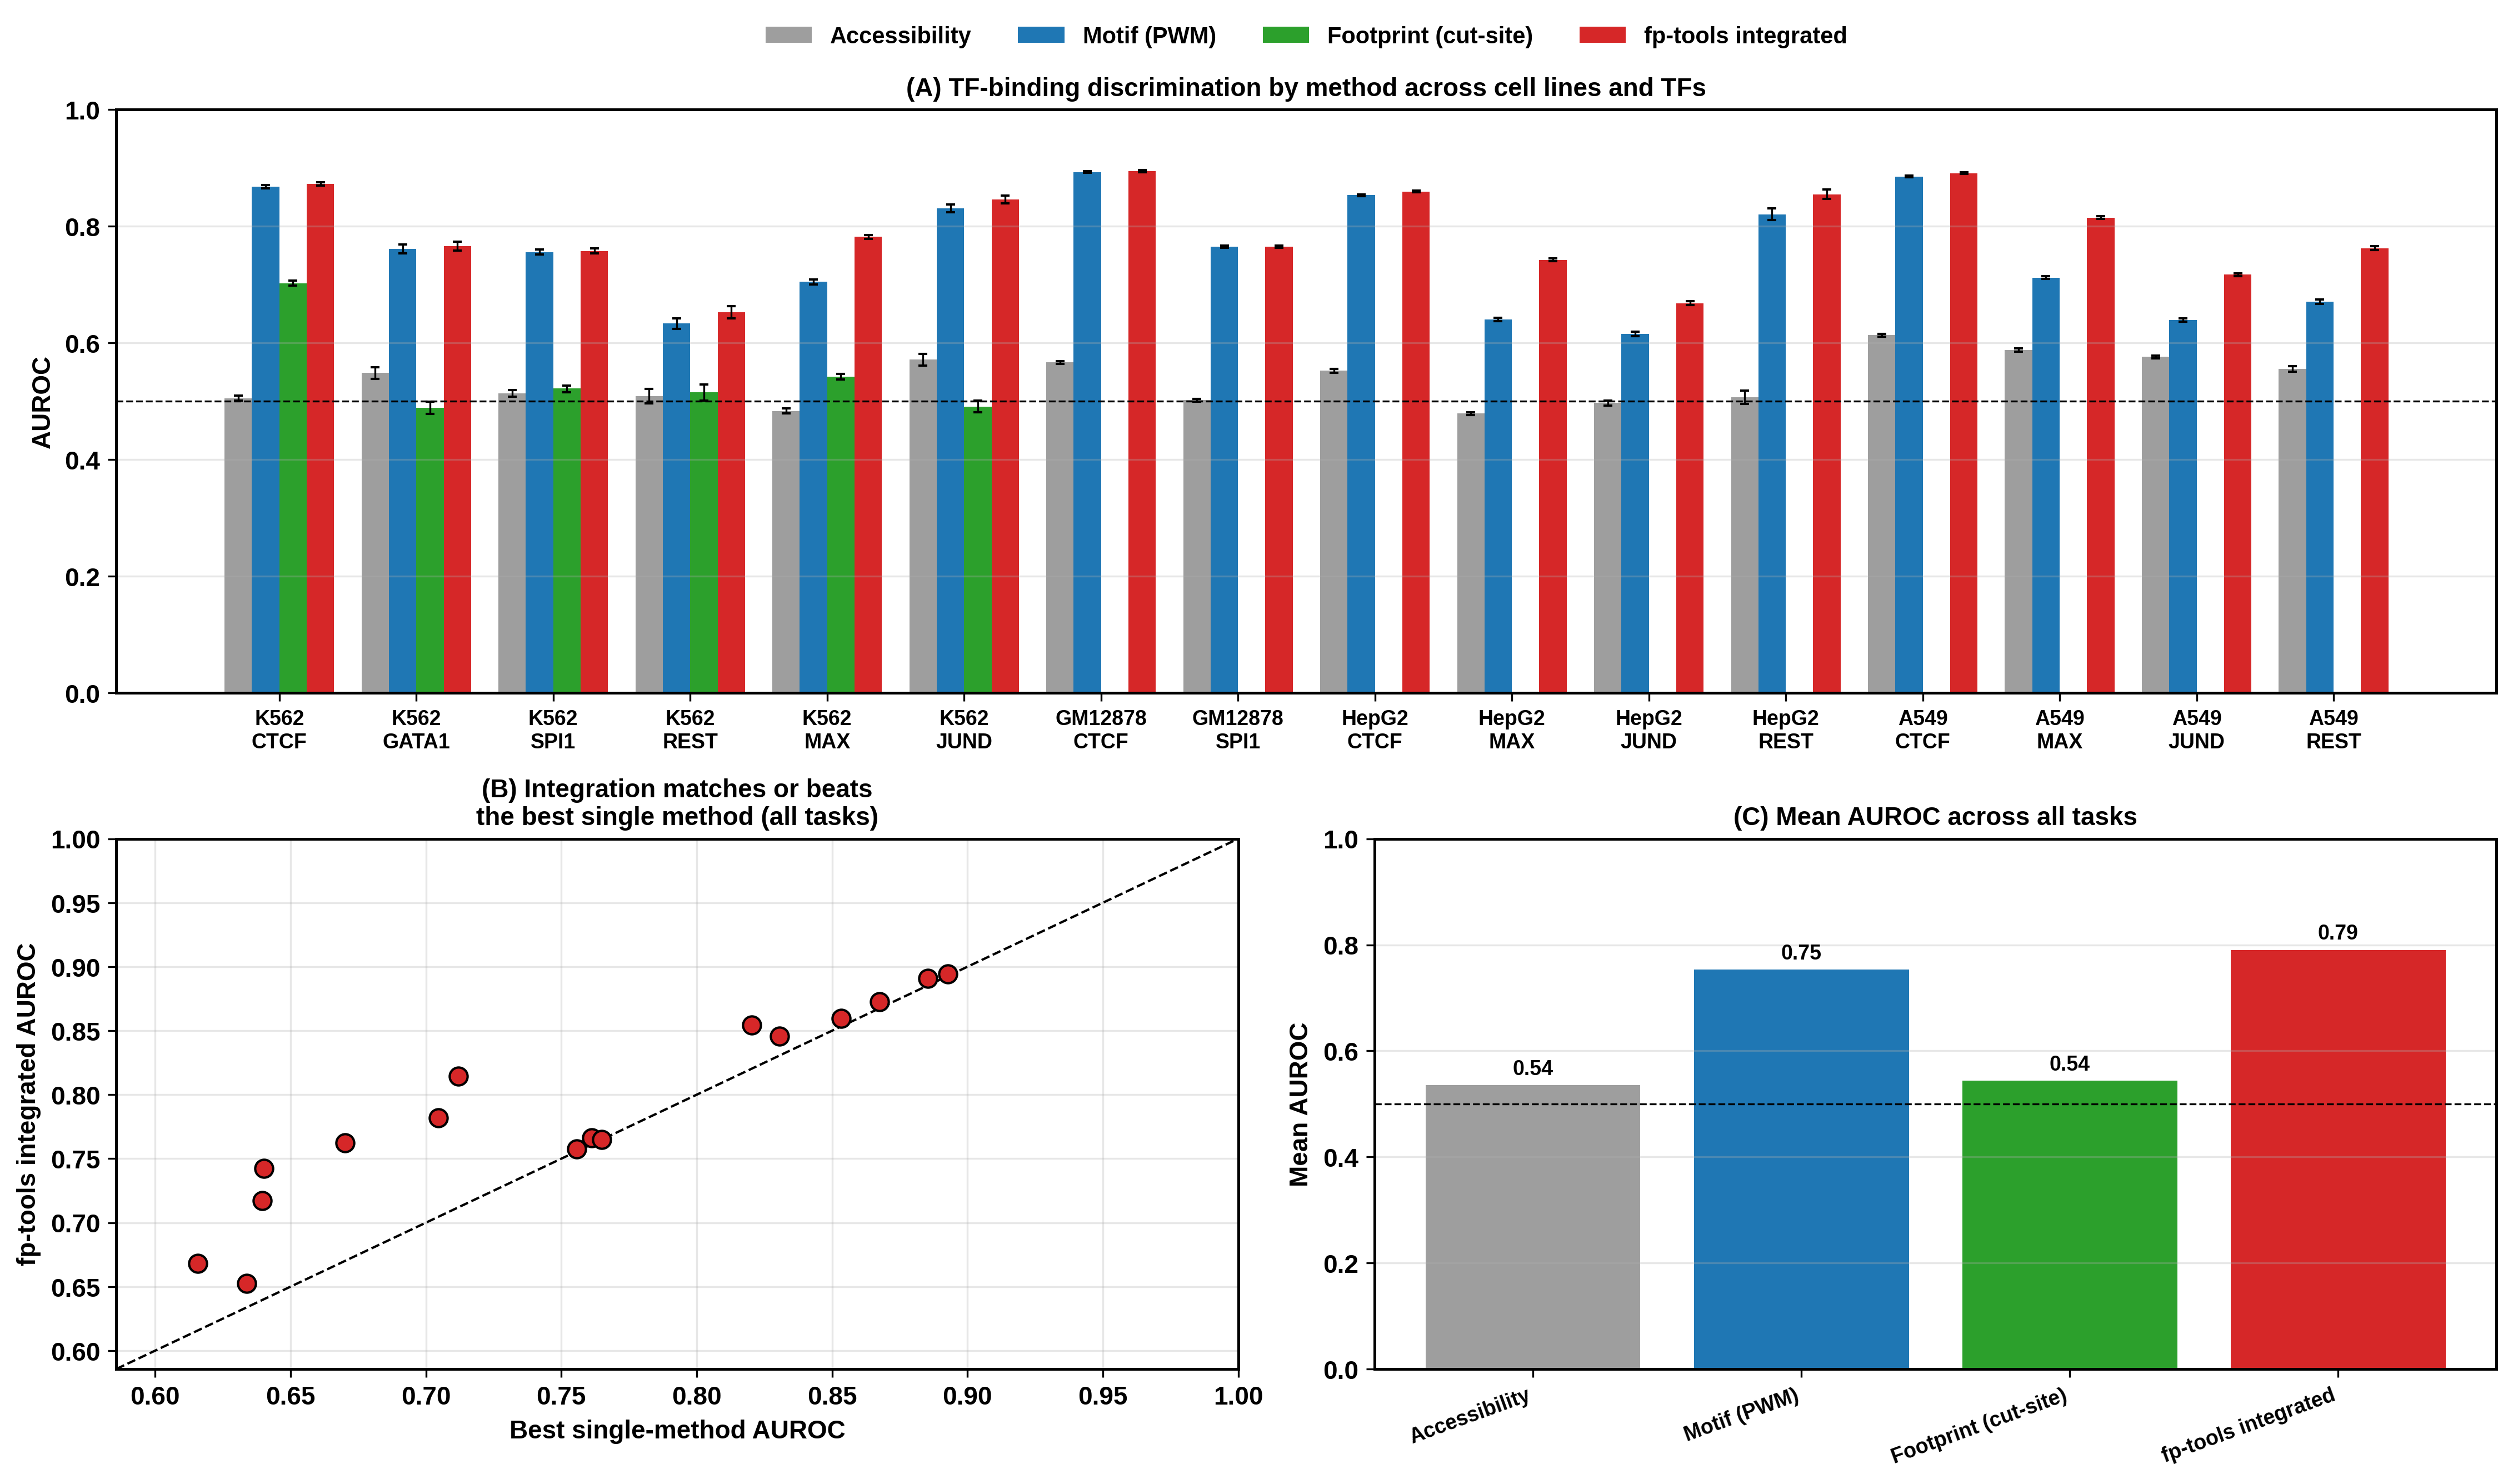
\includegraphics[width=\textwidth]{figures/method_comparison_multi.png}
\caption{Multi-method benchmark across three ENCODE cell lines and 12 cell--TF
tasks. Panel A compares per-task AUROC for raw accessibility, motif-only scoring,
cut-site footprint scoring where available, and the integrated \texttt{fp-tools}
model. Panel B compares the integrated model with the best single-method score for
each task. Panel C summarizes mean AUROC by method. Generated by
\texttt{paper/scripts/plot\_method\_comparison\_multi.py}.\label{fig:method_multi}}
\end{figure}

\subsection{Footprinting Requires Cut-Site Resolution}

Footprinting infers occupancy from a local depletion of Tn5 insertions at the bound
site, flanked by hyper-accessible edges. We tested this directly on K562 CTCF
(chromosome~4) by computing a footprint-occupancy score at each peak's best CTCF
motif match---the mean signal in the flanks minus the mean signal at the motif
site---using two different signal representations
(Figure~\ref{fig:footprint}). On a smoothed fold-change-over-control coverage
track the score is uninformative and in fact inverted (AUROC $=0.24$), because
coverage is \emph{enriched}, not depleted, at bound accessible sites. When the same
score is computed from base-resolution Tn5 cut sites derived from the ATAC BAM, it
recovers a genuine footprint signal (AUROC $=0.68$, 95\% CI $0.65$--$0.70$)---a
large gain that arises purely from using the correct, cut-site-resolution signal
that \texttt{fp-tools}' bias-correction and footprint-scoring pipeline is built to
produce. For CTCF, whose long motif is already highly predictive, the cut-site
footprint is an orthogonal but weaker line of evidence and does not exceed the motif
score; footprinting is expected to contribute most where motifs are weak or where
condition-specific occupancy changes are the question, which the differential
binding and replicate-aware modules target.

\begin{figure}[H]
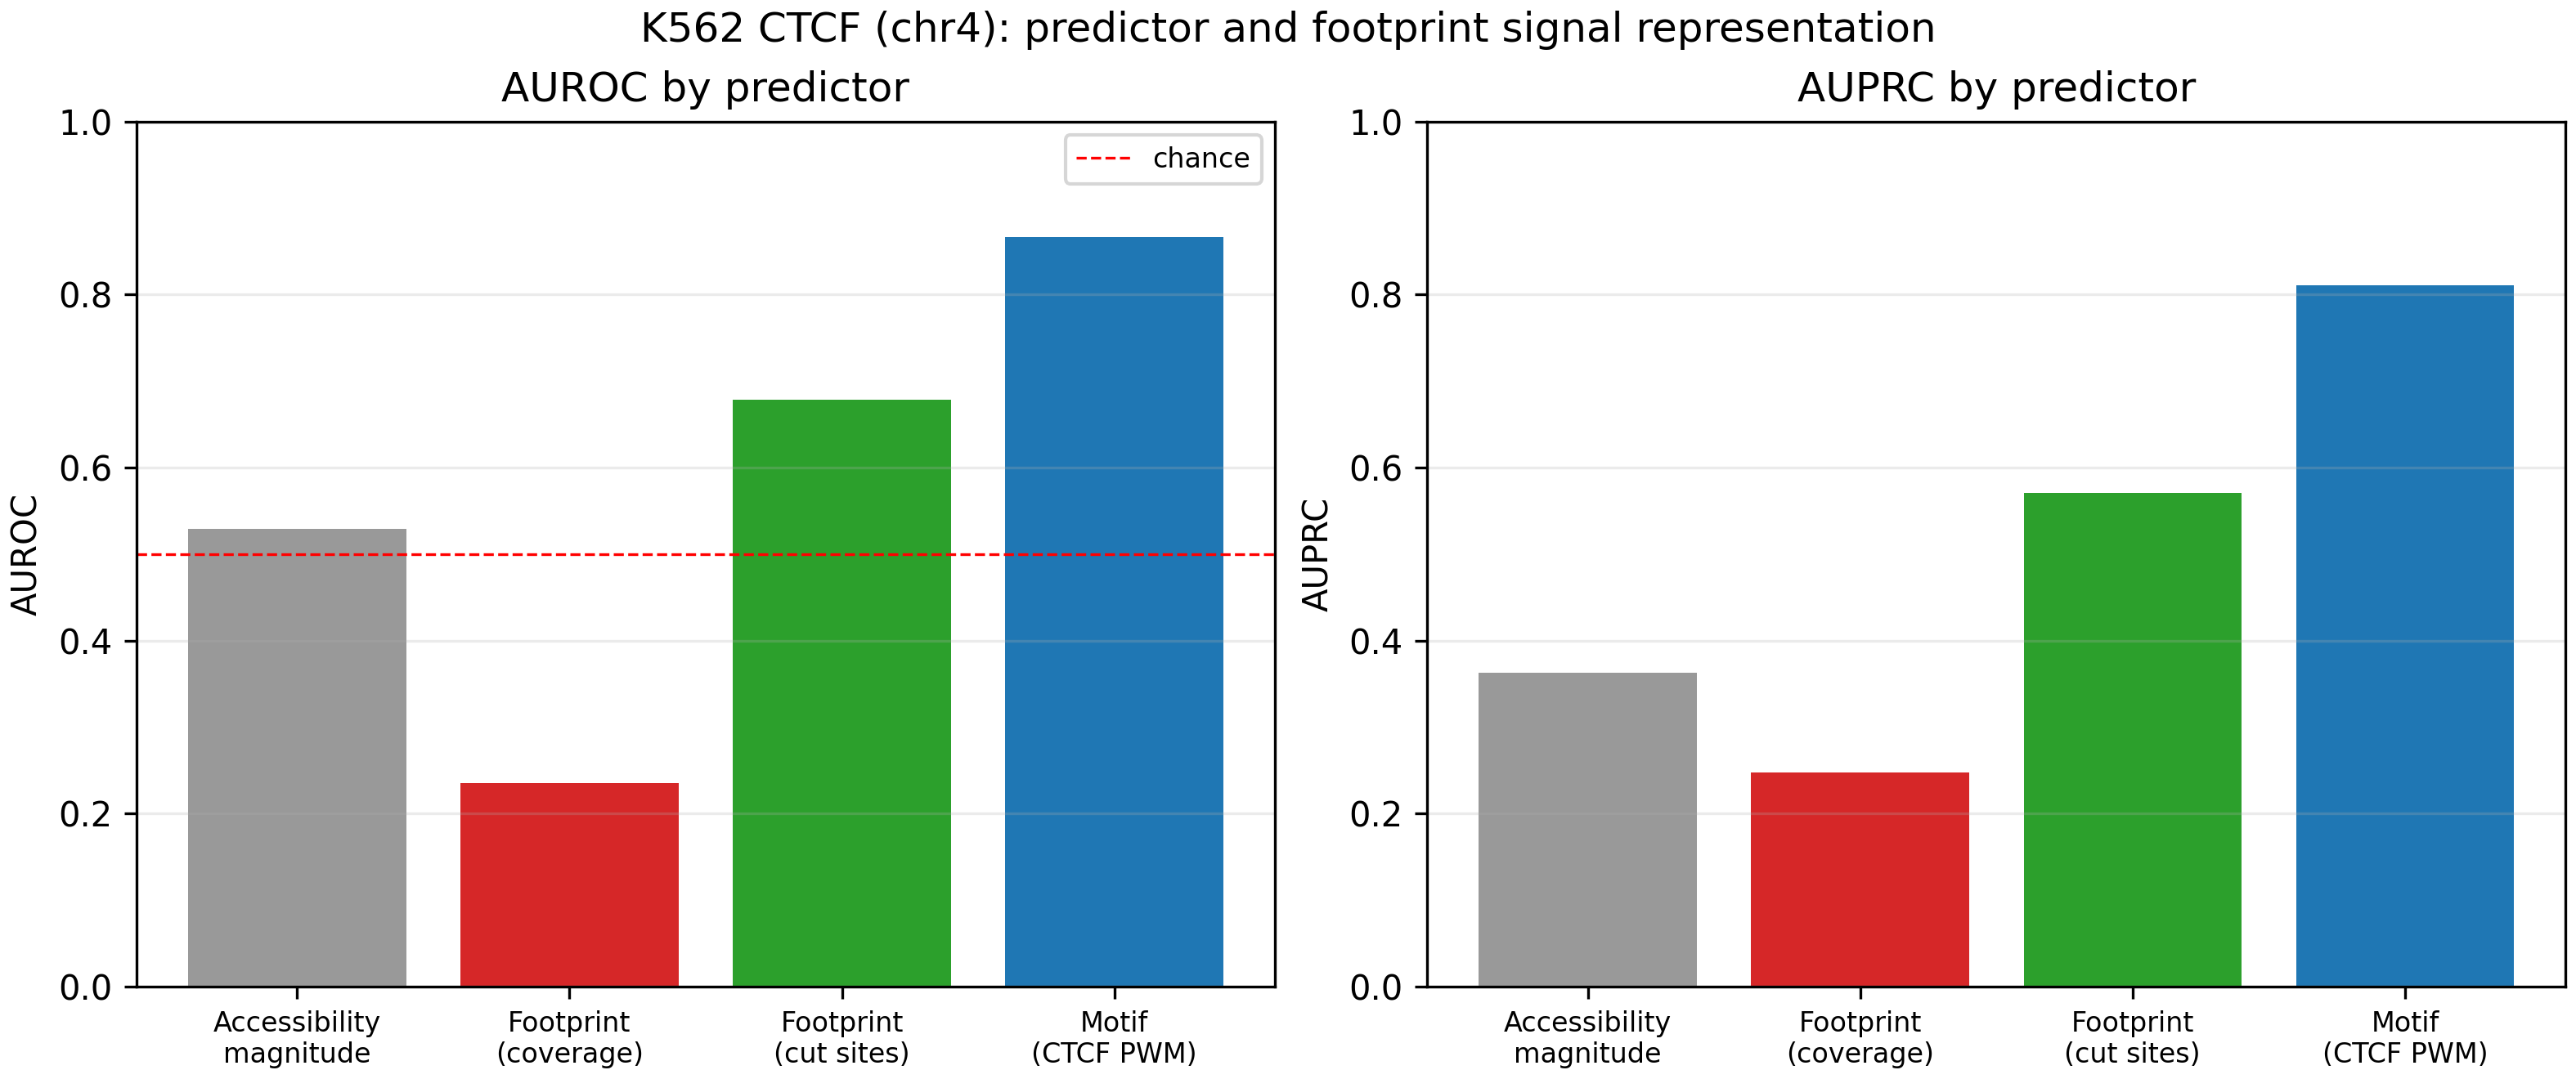
\includegraphics[width=\textwidth]{figures/footprint_representation.png}
\caption{Predictor comparison for K562 CTCF (chromosome~4). A footprint-occupancy
score is informative only at Tn5 cut-site resolution (green, AUROC $0.68$); the same
score on smoothed coverage is inverted and uninformative (red, $0.24$). Raw
accessibility (grey) is near chance and the CTCF motif (blue) is the single
strongest predictor.\label{fig:footprint}}
\end{figure}

%==================================================================
\section{Discussion}
%==================================================================

\texttt{fp-tools} occupies a deliberate position in the regulatory-genomics tool
landscape: rather than introducing a single new algorithm, it integrates
established classical footprinting with modern multiscale, supervised, de novo,
and variant-oriented capabilities inside one reproducible, testable package. Its
comparative strengths are interface consistency, deterministic regression
coverage, and a conservative extension model in which new science is opt-in and
non-disruptive. These properties target precisely the friction that slows applied
ATAC-seq analysis and cross-method benchmarking today.

We do not claim parity with deep sequence-to-profile models on tasks where learned
base-resolution sequence features dominate; ChromBPNet-class models and their
attribution-based interpreters remain state of the art for sequence-driven
occupancy and variant-effect prediction~\cite{chrombpnet2024}. \texttt{fp-tools}
instead aims to make classical and tabular-supervised analyses reproducible,
composable, and easy to benchmark against such models on shared labels. The
multiscale, competition-decomposition, and replicate-uncertainty modules are
pragmatic additions grounded in the available signal: in particular, the
replicate-aware standard error is reconstructed from reported $p$-values rather
than from per-replicate scores, so it should be read as a calibrated uncertainty
heuristic rather than a full hierarchical model, and per-replicate inputs would
enable a stronger formulation in future work.

Limitations include the chromosome-4 scope of the current pilot benchmark, the
dependence of larger public-benchmark results on external data acquisition and
comparator execution, which are intentionally kept outside version control for
size and licensing reasons; the tabular supervised models
trade base-resolution sequence modeling for transparency and speed; and several
roadmap items (attribution-based discovery, RNA-prior weighting for pseudobulk,
hierarchical differential binding) are scaffolded but not yet fully realized.
These are natural directions for subsequent releases.

%==================================================================
\section{Conclusions}
%==================================================================

We presented \texttt{fp-tools}, a standalone, reproducible command-line platform
that unifies classical ATAC-seq footprinting with opt-in multiscale, supervised,
motif-discovery, variant-scoring, pseudobulk, replicate-uncertainty, and
competition-decomposition modules. By keeping core workflows stable and
test-covered while adding new scientific behavior as composable, independently
validated modules---and by pairing them with a tiered public-data benchmark and
figure infrastructure---the package lowers the barrier to standardized,
benchmarkable regulatory-genomics analysis. Future work will complete whole-genome
or chromosome-held-out public biological benchmarks, strengthen the supervised and
hierarchical differential-binding models, and integrate attribution-based
discovery.

\vspace{6pt}

\authorcontributions{Conceptualization, Y.L. and C.Y.; methodology, Y.L.; software,
Y.L.; validation, Y.L.; formal analysis, Y.L.; investigation, Y.L.; data curation,
Y.L.; writing---original draft preparation, Y.L.; writing---review and editing, Y.L.
and C.Y.; visualization, Y.L.; supervision, C.Y.; project administration, C.Y.;
funding acquisition, C.Y. All authors have read and agreed to the published version
of the manuscript.}

\funding{This research received no external funding.}

\institutionalreview{Not applicable. This study used only publicly available,
de-identified datasets and did not involve new experiments on humans or animals.}

\informedconsent{Not applicable.}

\dataavailability{\texttt{fp-tools} is openly available at
\url{https://github.com/oncologylab/fp-tools}. All benchmark manifests, schemas,
analysis scripts, and figure generators are included in the repository. Public
input datasets are obtained from the ENCODE Project~\cite{encode2012} and motif
databases (e.g., JASPAR~\cite{jaspar2026}) via the included discovery and download
scripts; large raw and processed data and full benchmark outputs are regenerated
from the committed manifests rather than stored in version control.}

\acknowledgments{The author thanks the ENCODE Project Consortium and the
maintainers of the open-source tools referenced in this work for making their data
and software publicly available.}

\conflictsofinterest{The author declares no conflicts of interest.}

%==================================================================
\begin{thebibliography}{99}

\bibitem{buenrostro2013}
Buenrostro, J.D.; Giresi, P.G.; Zaba, L.C.; Chang, H.Y.; Greenleaf, W.J.
Transposition of native chromatin for fast and sensitive epigenomic profiling of
open chromatin, DNA-binding proteins and nucleosome position. \textit{Nat.
Methods} \textbf{2013}, \textit{10}, 1213--1218.

\bibitem{bentsen2020}
Bentsen, M.; Goymann, P.; Schultheis, H.; Klee, K.; Petrova, A.; Wiegandt, R.;
Fust, A.; Preussner, J.; Kuenne, C.; Braun, T.; et al. ATAC-seq footprinting
unravels kinetics of transcription factor binding during zygotic genome
activation. \textit{Nat. Commun.} \textbf{2020}, \textit{11}, 4267.

\bibitem{li2019hint}
Li, Z.; Schulz, M.H.; Look, T.; Begemann, M.; Zenke, M.; Costa, I.G. Identification
of transcription factor binding sites using ATAC-seq. \textit{Genome Biol.}
\textbf{2019}, \textit{20}, 45.

\bibitem{hu2024print}
Hu, Y.; et al. Multiscale footprinting reveals the regulatory grammar of chromatin
accessibility (PRINT/scPrinter). \textit{Nature/bioRxiv} \textbf{2024}.

\bibitem{cazares2023maxatac}
Cazares, T.A.; Rizvi, F.W.; Iyer, B.; Chen, X.; Kotliar, M.; Bejjani, A.T.;
Wayman, J.A.; Donmez, O.; Wronowski, B.; Parameswaran, S.; et al. maxATAC:
Genome-scale transcription-factor binding prediction from ATAC-seq with deep neural
networks. \textit{PLoS Comput. Biol.} \textbf{2023}, \textit{19}, e1010863.

\bibitem{chrombpnet2024}
Pampari, A.; et al. ChromBPNet: base-resolution models of chromatin accessibility
reveal the sequence basis of TF binding and variant effects.
\textit{bioRxiv/Nature} \textbf{2024}.

\bibitem{encode2012}
The ENCODE Project Consortium. An integrated encyclopedia of DNA elements in the
human genome. \textit{Nature} \textbf{2012}, \textit{489}, 57--74.

\bibitem{jaspar2026}
Rauluseviciute, I.; et al. JASPAR 2026: update of the open-access database of
transcription factor binding profiles. \textit{Nucleic Acids Res.} \textbf{2026}.

\end{thebibliography}

\end{document}
